\documentclass[journal,12pt,onecolumn]{IEEEtran}
\usepackage{cite}
\usepackage{graphicx}
\usepackage{amsmath,amssymb,amsfonts,amsthm}
\usepackage{algorithmic}
\usepackage{graphicx}
\usepackage{textcomp}
\usepackage{tfrupee}
\usepackage{xcolor}
\usepackage{txfonts}
\usepackage{listings}
\usepackage{enumitem}
\usepackage{mathtools}
\usepackage{gensymb}
\usepackage{comment}
\usepackage[breaklinks=true]{hyperref}
\usepackage{tkz-euclide} 
\usepackage{listings}
\usepackage{gvv}                                        
%\def\inputGnumericTable{}                                 
\usepackage[latin1]{inputenc} 
\usetikzlibrary{arrows.meta, positioning}
\usepackage{xparse}
\usepackage{color}                                            
\usepackage{array}                                            
\usepackage{longtable}                                       
\usepackage{calc}                                             
\usepackage{multirow}
\usepackage{multicol}
\usepackage{hhline}                                           
\usepackage{ifthen}                                           
\usepackage{lscape}
\usepackage{tabularx}
\usepackage{array}
\usepackage{float}
\newtheorem{theorem}{Theorem}[section]
\newtheorem{problem}{Problem}
\newtheorem{proposition}{Proposition}[section]
\newtheorem{lemma}{Lemma}[section]
\newtheorem{corollary}[theorem]{Corollary}
\newtheorem{example}{Example}[section]
\newtheorem{definition}[problem]{Definition}
\newcommand{\BEQA}{\begin{eqnarray}}
\newcommand{\EEQA}{\end{eqnarray}}
\usepackage{float}
%\newcommand{\define}{\stackrel{\triangle}{=}}
\theoremstyle{remark}
\usepackage{circuitikz}
\usepackage{tikz}
% Marks the beginning of the document
\begin{document}
\title{2025-XH-'1-65'}
\author{EE25BTECH11020 - Darsh Pankaj Gajare}
\maketitle
\begin{enumerate}

  \item Here are two analogous groups, Group -I and Group -II, that list words in their decreasing order of intensity. Identify the missing word in Group -II.  

  Group -I: Abuse $\to$ Insult $\to$ Ridicule  

  Group -II: \rule{2cm}{0.15mm} $\to$ Praise $\to$ Appreciate  
\hfill $\brak{GATE\ EE\ 2025}$
  \begin{multicols}{4}
  \begin{enumerate}
    \item Extol
    \item Prize
    \item Appropriate
    \item Espouse
  \end{enumerate}
  \end{multicols}

  \item Had I learnt acting as a child, I \rule{2cm}{0.15mm} a famous film star. Select the most appropriate option to complete the above sentence.  
\hfill $\brak{GATE\ EE\ 2025}$
  \begin{multicols}{4}
  \begin{enumerate}
    \item will be
    \item can be
    \item am going to be
    \item could have been
  \end{enumerate}
  \end{multicols}

  \item The 12 musical notes are given as C, C\#, D, D\#, E, F, F\#, G, G\#, A, A\#, and B.  
  Frequency of each note is $\sqrt{2}^{12}$ times the frequency of the previous note.  
  If the frequency of the note C is 130.8 Hz, then the ratio of frequencies of notes F\# and C is:  
\hfill $\brak{GATE\ EE\ 2025}$
  \begin{multicols}{4}
  \begin{enumerate}
    \item $\sqrt{2^{6}}$
    \item $\sqrt{2}$
    \item $\sqrt{2^{4}}$
    \item 2
  \end{enumerate}
  \end{multicols}
  \item The following figures show three curves generated using an iterative algorithm.  
  The total length of the curve generated after 'Iteration $n$' is:  

  Note: The figures shown are representative.  
  \hfill $\brak{GATE\ EE\ 2025}$
\begin{figure}[H]
\centering
\caption{Q4}
\label{Q4}
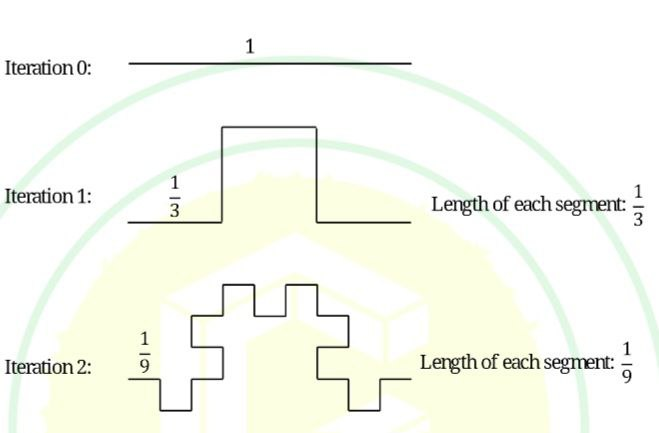
\includegraphics[scale=0.5]{figs/Q4.jpg}
\end{figure}

  \begin{multicols}{4}
  \begin{enumerate}
    \item $\brak{\frac{5}{3}}^n$
    \item $\frac{5}{3^{n}}$
    \item $\brak{\frac{5}{3}}^{2n}$
    \item $\brak{\frac{5}{3}}^{n\brak{2n-1}}$
  \end{enumerate}
  \end{multicols}

  \item Which one of the following plots represents $f(x) = -\frac{|x|}{x}$, where $x$ is a non-zero real number?  

  Note: The figures shown are representative.  
\hfill $\brak{GATE\ EE\ 2025}$
  \begin{multicols}{4}
  \begin{enumerate}
    \item \begin{figure}[H]
\centering
\caption{Q5a}
\label{Q5a}
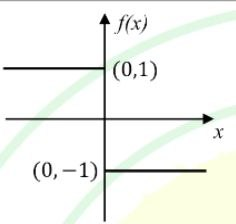
\includegraphics[scale=0.5]{figs/Q5a.jpg}
\end{figure}
    \item \begin{figure}[H]
\centering
\caption{Q5b}
\label{Q5b}
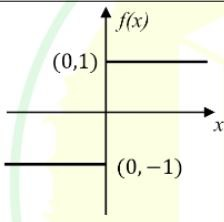
\includegraphics[scale=0.5]{figs/Q5b.jpg}
\end{figure}
    \item \begin{figure}[H]
\centering
\caption{Q5c}
\label{Q5c}
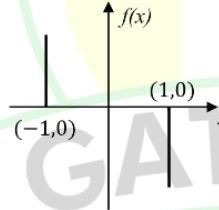
\includegraphics[scale=0.5]{figs/Q5c.jpg}
\end{figure}
    \item \begin{figure}[H]
\centering
\caption{Q5c}
\label{Q5c}
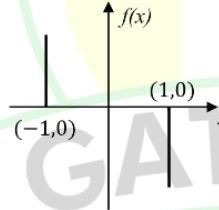
\includegraphics[scale=0.5]{figs/Q5c.jpg}
\end{figure}
  \end{enumerate}
  \end{multicols}

  \item Identify the option that has the most appropriate sequence such that a coherent paragraph is formed:  

  P. Over time, such adaptations lead to significant evolutionary changes with the potential to shape the development of new species.  
  Q. In the natural world, organisms constantly adapt to their environments in response to challenges and opportunities.  
  R. This process of adaptation is driven by the principle of natural selection, where favorable traits increase an organism's chances of survival and reproduction.  
  S. As environments change, organisms that can adapt their behavior, structure and physiology to such changes are more likely to survive.  
\hfill $\brak{GATE\ EE\ 2025}$
  \begin{multicols}{4}
  \begin{enumerate}
    \item P $\to$ Q $\to$ R $\to$ S
    \item Q $\to$ S $\to$ R $\to$ P
    \item R $\to$ S $\to$ Q $\to$ P
    \item S $\to$ P $\to$ R $\to$ Q
  \end{enumerate}
  \end{multicols}

  \item A stick of length $1\,m$ is broken at two locations at distances $b_1$ and $b_2$ from the origin $(0)$, with $0<b_1<b_2<1$. Which one is NOT a necessary condition for forming a triangle using the three pieces? 
  \begin{figure}[H]
\centering
\caption{Q7}
\label{Q7}
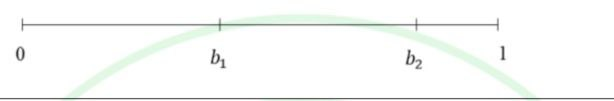
\includegraphics[scale=0.5]{figs/Q7.jpg}
\end{figure}
\hfill $\brak{GATE\ EE\ 2025}$
\begin{enumerate}
\begin{multicols}{2}
\item $b_1 < 0.5$
\item $b_2 > 0.5$
\item $b_2 < b_1 + 0.5$
\item $b_1 + b_2 < 1$
\end{multicols}
\end{enumerate}

\item Eight students $P,Q,R,S,T,U,V,W$ are playing musical chairs in a circle (clockwise). After 1st round, 4th behind $P$ leaves; after 2nd round, 5th behind $Q$ leaves; after 3rd round, 3rd behind $V$ leaves; after 4th round, 4th behind $U$ leaves. Who are left after the 4th round? 
\begin{figure}[H]
\centering
\caption{Q8}
\label{Q8}
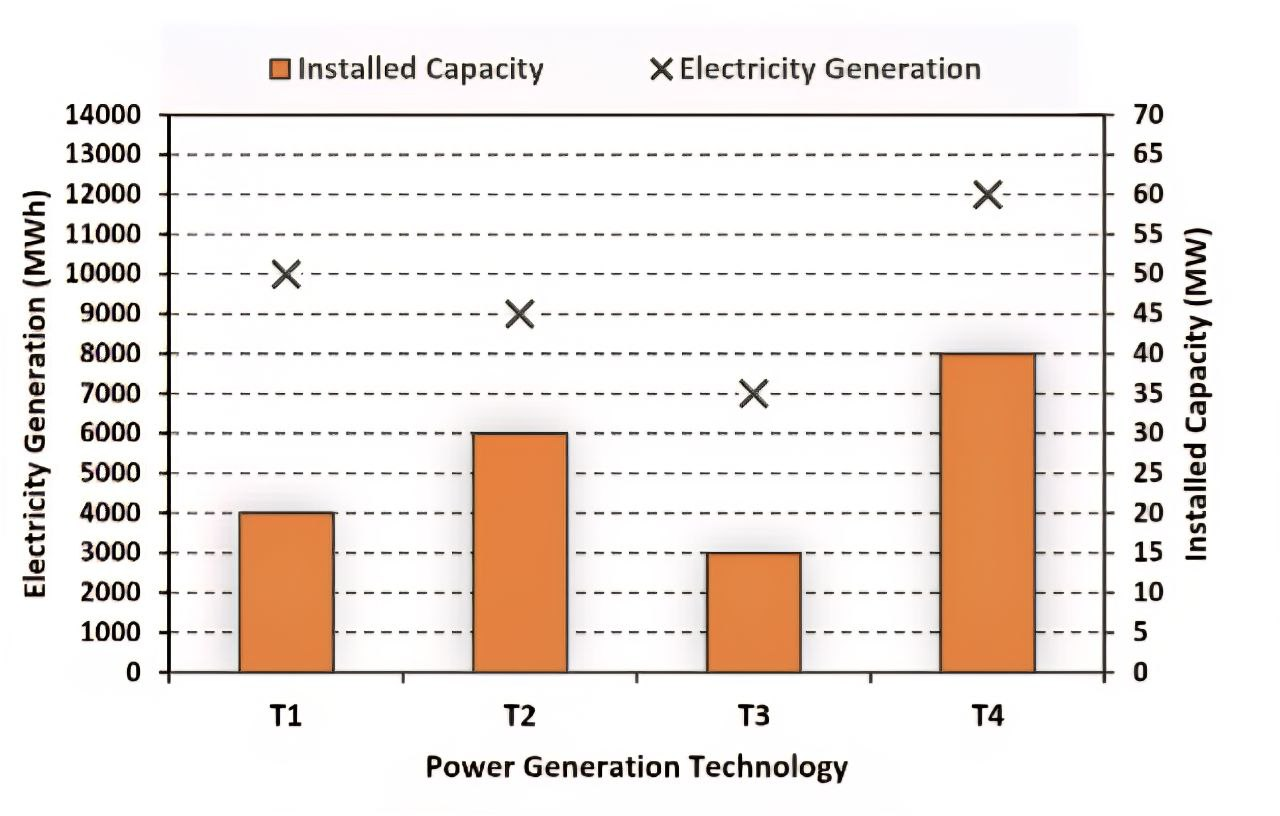
\includegraphics[scale=0.15]{figs/Q8.jpg}
\end{figure}
\hfill $\brak{GATE\ EE\ 2025}$
\begin{enumerate}
\begin{multicols}{2}
\item P, T, Q, S
\item V, P, T, Q
\item W, R, Q, V
\item Q, T, V, W
\end{multicols}
\end{enumerate}

\item The table lists the top 5 nations according to the number of gold medals, also silver and bronze. Based only on this data, which statement is INCORRECT? 
\begin{table}[H]
\centering
\begin{tabular}{|c|c|c|c|}
\hline
\text{Nation} & \text{Gold} & \text{Silver} & \text{Bronze} \\
\hline
\text{USA} & 40 & 44 & 41 \\
\hline
\text{Canada} & 39 & 27 & 24 \\
\hline
\text{Japan} & 20 & 12 & 13 \\
\hline
\text{Australia} & 17 & 19 & 16 \\
\hline
\text{France} & 16 & 26 & 22 \\
\hline
\end{tabular}

\caption{Q9}
\label{Q9}
\end{table}

  \hfill $\brak{GATE\ EE\ 2025}$
\begin{enumerate}
\begin{multicols}{2}
\item France will occupy third place if list is based on total medals.
\item The order of top two nations does not change if list is based on total medals.
\item USA and Canada together have less than 50\% of total medals.
\item Canada has won twice as many total medals as Japan.
\end{multicols}
\end{enumerate}
  \item An organization allows its employees to work independently on consultancy projects but charges an overhead on the consulting fee. The overhead is 20\% of the consulting fee, if the fee is up to \rupee5,00,000. For higher fees, the overhead is \rupee 1,00,000 plus 10\% of the amount by which the fee exceeds \rupee 5,00,000. The government charges a Goods and Services Tax of 18\% on the total amount $\brak{the\ consulting\ fee\ plus\ the\ overhead}$. An employee of the organization charges this entire amount, i.e., the consulting fee, overhead, and tax, to the client. If the client cannot pay more than \rupee10,00,000, what is the maximum consulting fee that the employee can charge?  

  \begin{multicols}{4}
  \begin{enumerate}
    \item \rupee 7,01,438
    \item \rupee 7,24,961
    \item \rupee 7,51,232
    \item \rupee 7,75,784
  \end{enumerate}
  \end{multicols}
% Continuing enumerate from Q.10

\item Which one of the following numbers is odd one out? \\
31541,\;42651,\;53791,\;64871,\;75981
\hfill $\brak{GATE\ EE\ 2025}$
\begin{enumerate}
\begin{multicols}{4}
\item 31541
\item 42651
\item 53791
\item 75981
\end{multicols}
\end{enumerate}

\item Ankit, Arun, and Ankur have one apple each. Ankur also has one banana. Alam has one mango and one kiwi. Ankit has just bought one pineapple. \\
Who has the least number of fruit(s)?
\hfill $\brak{GATE\ EE\ 2025}$
\begin{enumerate}
\begin{multicols}{4}
\item Ankit
\item Arun
\item Ankur
\item Alam
\end{multicols}
\end{enumerate}

\item If each vowel in the word \textbf{RESIDE} is changed to its previous letter in the English alphabet and each consonant is changed to the next letter in the English alphabet, which one of the following options will be the third from the right?
\hfill $\brak{GATE\ EE\ 2025}$
\begin{enumerate}
\begin{multicols}{4}
\item T
\item D
\item S
\item H
\end{multicols}
\end{enumerate}

\item Vipul, Ahmad, Santosh, and David are playing Carrom. Vipul and Ahmad are partners sitting opposite to each other. David faces towards South. If Vipul faces towards West, then who faces towards the North?
\hfill $\brak{GATE\ EE\ 2025}$
\begin{enumerate}
\begin{multicols}{4}
\item Alam
\item Santosh
\item David
\item Vipul
\end{multicols}
\end{enumerate}

\item Consider the following sentence: \\
``What the country needs \rule{2cm}{0.4pt} accordingly.'' \\
First and last parts of the sentence are given. P, Q, R, and S are the remaining parts of the sentence, not necessarily in that order. \\
P: and change tactics \\
Q: who would encourage players \\
R: are coaches and officials \\
S: to read the game as it progresses
\hfill $\brak{GATE\ EE\ 2025}$
\begin{enumerate}
\begin{multicols}{4}
\item QSPR
\item RQSP
\item RQPS
\item SPRQ
\end{multicols}
\end{enumerate}

\item A car started from city P at 9:40 AM. The time taken for the car to reach city Q is 4 hours and 50 minutes. The time of arrival of the car at city Q is:
\hfill $\brak{GATE\ EE\ 2025}$
\begin{enumerate}
\begin{multicols}{4}
\item 15:10 Hours
\item 14:20 Hours
\item 14:30 Hours
\item 14:10 Hours
\end{multicols}
\end{enumerate}

\item P is three years younger than R but one year older than S. S is one year older than Q but 4 years younger than R. R is 15 years old. The age of Q is \rule{1cm}{0.4pt} years. 
\hfill $\brak{GATE\ EE\ 2025}$

\item In a certain code language, ATTITUDE is written as \textbf{TAUJUEDU} and CHILDREN is written as \textbf{HCJMENER}. How is LANGUAGE written in that code language?
\hfill $\brak{GATE\ EE\ 2025}$
\begin{enumerate}
\begin{multicols}{4}
\item ALOHVEGA
\item ALHOVAGA
\item LAVOHEGA
\item ALHOVGEA
\end{multicols}
\end{enumerate}

\item The table shows the data of 450 candidates who appeared in the examination of three subjects -- Social Science, Mathematics, and Science. 
\begin{table}[H]
\centering
\begin{tabular}{|c|c|}
\hline
\textbf{Particulars} & \textbf{Number of candidates} \\
\hline
Passed in all the three subjects & 167 \\
Failed in all the three subjects & 60 \\
Failed in Social Science subject & 175 \\
Failed in Mathematics subject & 199 \\
Failed in Science subject & 191 \\
Passed in only Social Science subject & 62 \\
Passed in only Mathematics subject & 48 \\
Passed in only Science subject & 52 \\
\hline
\end{tabular}

\caption{Q19}
\label{Q19}
\end{table}
How many candidates have passed in at least one subject?
\hfill $\brak{GATE\ EE\ 2025}$
\begin{enumerate}
\begin{multicols}{4}
\item 48
\item 162
\item 390
\item 425
\end{multicols}
\end{enumerate}

\item If $\times$ means $+$, $+$ means $\div$, $-$ means $\times$, and $\div$ means $-$, then the value of the expression \\
$28 - 42 \div 7 + 5 \times 3$ is equal to:
\hfill $\brak{GATE\ EE\ 2025}$
\begin{enumerate}
\begin{multicols}{4}
\item 13
\item 15
\item 17
\item 19
\end{multicols}
\end{enumerate}
% Continuing enumerate from Q.20

\item Given a series $5, 8, 11, 14, \dots$ \\
If the $n^{th}$ term of the given series is $320$, then $n$ (where $n \geq 1$) is:
\hfill $\brak{GATE\ EE\ 2025}$
\begin{enumerate}
\begin{multicols}{4}
\item 104
\item 105
\item 106
\item 107
\end{multicols}
\end{enumerate}

\item Suppose your last year taxable income was Rs.\ 22000. Due to hike in salary, your taxable income this year is Rs.\ 34200. The details for tax calculation are: \\
\begin{table}[H]
\centering
%22
\begin{tabular}{|l|l|}
\hline
\textbf{Income range (Rs.)} & \textbf{Tax slab (Rs.)} \\
\hline
0 to 5000 & 2\% of income \\
\hline
Greater than 5000 to 10000 & 100 + 3\% of income over 5000 \\
\hline
Greater than 10000 to 20000 & 250 + 5\% of income over 10000 \\
\hline
Greater than 20000 to 30000 & 750 + 8\% of income over 20000 \\
\hline
Greater than 30000 to 50000 & 1550 + 10\% of income over 30000 \\
\hline
Greater than 50000 to 100000 & 3550 + 20\% of income over 50000 \\
\hline
\end{tabular}

\caption{Q22}
\label{Q22}
\end{table}

What is the additional tax to be paid this year compared to last year?
\hfill $\brak{GATE\ EE\ 2025}$
\begin{enumerate}
\begin{multicols}{4}
\item 1970
\item 1060
\item 910
\item 420
\end{multicols}
\end{enumerate}

\item Anand, Hari, and Chris are engaged in one of the three occupations - clerk, teacher, and plumber, not necessarily in that order. Each person is assigned only one type of occupation. Clerk is Chris's cousin. Hari lives next door to the plumber. Anand, who knows more facts than the teacher, has to drive more than 1 hour to reach Hari's home. \\
Which one is correct?
\hfill $\brak{GATE\ EE\ 2025}$
\begin{enumerate}
\begin{multicols}{2}
\item Anand is teacher and Chris is clerk.
\item Hari is clerk and Anand is plumber.
\item Chris is teacher and Hari is clerk.
\item Anand is clerk and Chris is plumber.
\end{multicols}
\end{enumerate}

\item Many countries are facing water shortage crises in the past few years. A UN report has named India among the worst countries for poor quality of water. The report ranks 122 countries according to water quality as well as commitment to improve. Some countries in Europe are considered worst because of ground water. Rain failed in some parts of India; Rajasthan, Madhya Pradesh, and Andhra Pradesh were affected by drought. People without water turn desperate and violent. Consequently, food godowns were attacked in some states. \\
Which statement(s) is/are correct?
\hfill $\brak{GATE\ EE\ 2025}$
\begin{enumerate}
\begin{multicols}{2}
\item There is no proof that India is affected by poor quality of water.
\item A few European countries are suffering due to occurrence of drought.
\item Lack of access to water can lead to social unrest.
\item Intense shortage of water is visible in some states of India.
\end{multicols}
\end{enumerate}

\item In the following figure, four overlapping shapes (rectangle, triangle, circle, hexagon) are given. The sum of the numbers which belong to only two overlapping shapes is \rule{2cm}{0.4pt}. \\
\begin{figure}[H]
\centering
\caption{Q25}
\label{Q25}
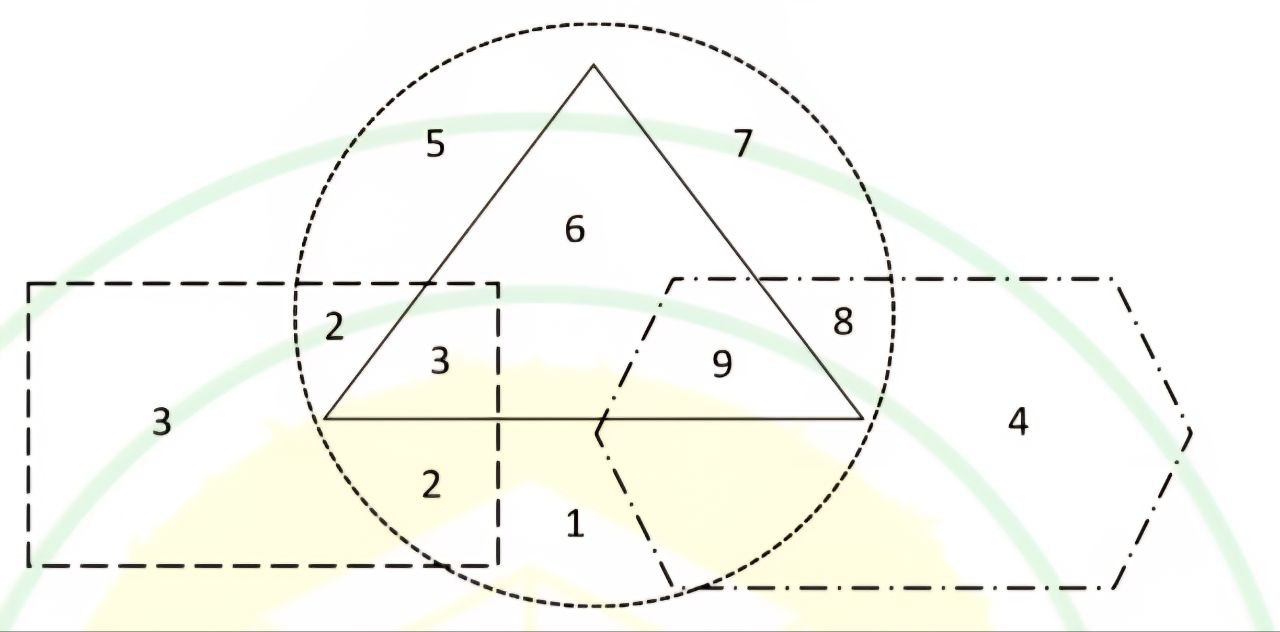
\includegraphics[scale=0.25]{figs/Q25.jpg}
\end{figure}
\hfill $\brak{GATE\ EE\ 2025}$

\item Consider a square field $ABCD$. The diagonal $AC$ is $50\,m$. The cost of laying grass is Rs.\ 5 per sq.m. \\
What is the total cost for laying grass in the field $ABCD$? (rounded off to 2 decimal places).
\hfill $\brak{GATE\ EE\ 2025}$

\item In the context of a perfectly competitive market, identify the statement that is \textbf{NOT CORRECT}.
\hfill $\brak{GATE\ EE\ 2025}$
\begin{enumerate}
\begin{multicols}{2}
\item Producing less than the competitive output lowers welfare.
\item Producing more than the competitive output lowers welfare.
\item The welfare is dependent on both price and the competitive output.
\item If a consumer values the last unit more than its marginal cost of production, producing an additional unit shall lower welfare.
\end{multicols}
\end{enumerate}

\item The demand function is given as
$
\log Q = \log A + 0.5 \log P
$
where $Q$ is quantity, $P$ is the unit price of the good and $A$ is a positive real number. The own price elasticity of demand is:
\hfill $\brak{GATE\ EE\ 2025}$
\begin{enumerate}
\begin{multicols}{2}
\item Perfectly elastic
\item Perfectly inelastic
\item Elastic
\item Inelastic
\end{multicols}
\end{enumerate}
\item Which one of the following is part of the unconventional monetary policy?
\hfill $\brak{GATE\ EE\ 2025}$
\begin{enumerate}
\begin{multicols}{2}
\item Repo rate
\item Quantitative easing
\item Fractional banking
\item Reverse Repo rate
\end{multicols}
\end{enumerate}

\item Which one of the following statements is \textbf{NOT CORRECT} in the context of Keynesian Absolute Income Hypothesis?
\hfill $\brak{GATE\ EE\ 2025}$
\begin{enumerate}
\begin{multicols}{2}
\item Average Propensity to Consume (APC) plus Average Propensity to Save (APS) is equal to one.
\item Marginal Propensity to Consume (MPC) is constant.
\item Average Propensity to Consume (APC) increases as income increases.
\item Marginal Propensity to Consume (MPC) plus Marginal Propensity to Save (MPS) is equal to one.
\end{multicols}
\end{enumerate}
% Continuing enumerate from Q.30

\item Let $f(x,y,z) = x^2 y^3 z$. Then,
$
x \frac{\partial f}{\partial x}(x,y,z) + y \frac{\partial f}{\partial y}(x,y,z) + z \frac{\partial f}{\partial z}(x,y,z) = ?
$
\hfill $\brak{GATE\ EE\ 2025}$
\begin{enumerate}
\begin{multicols}{2}
\item $f(x,y,z)$
\item $2f(x,y,z)$
\item $3f(x,y,z)$
\item $6f(x,y,z)$
\end{multicols}
\end{enumerate}

\item Let $f(x) = -3x^2(1-x) - 3x(1-x)^2 - (1-x)^3$. Then,
$
\frac{df(x)}{dx} = ?
$
\hfill $\brak{GATE\ EE\ 2025}$
\begin{enumerate}
\begin{multicols}{2}
\item $3x^2$
\item $3(1-x)^2$
\item $3x(1-x)$
\item $x$
\end{multicols}
\end{enumerate}

\item In the context of environmental cost-benefit analysis, which of the following statements is/are NOT CORRECT?
\hfill $\brak{GATE\ EE\ 2025}$
\begin{enumerate}
\begin{multicols}{2}
\item The discount rates do not impact the fixed and variable costs of the project but do impact the perceived benefits in monetary terms.
\item The analysis does not incorporate people's preferences for a policy.
\item The analysis is dependent on the choice of the discount rates.
\item The discount rates are not easily observable and choice is often subject to value judgements.
\end{multicols}
\end{enumerate}

\item Which of the following statements is/are CORRECT in the context of National Income Accounting?
\hfill $\brak{GATE\ EE\ 2025}$
\begin{enumerate}
\begin{multicols}{2}
\item Gross Domestic Product (GDP) is the sum of all factor payments.
\item Net Domestic Product (NDP) = GDP $-$ depreciation.
\item Gross National Product (GNP) = GDP $+$ net income from abroad.
\item Net National Product (NNP) = GNP $-$ GDP.
\end{multicols}
\end{enumerate}

\item Consider the following system of linear equations:
$
x + 2y + 3z = 0, \quad
2x + py = 0, \quad
3x + 2y + pz = 0
$
The value(s) of $p$ for which the system has infinitely many solutions is/are:
\hfill $\brak{GATE\ EE\ 2025}$
\begin{enumerate}
\begin{multicols}{2}
\item $p=1$
\item $p=2$
\item $p=6$
\item $p=12$
\end{multicols}
\end{enumerate}

\item Which of the following statements is/are CORRECT?
\hfill $\brak{GATE\ EE\ 2025}$
\begin{enumerate}
\begin{multicols}{2}
\item The difference between Human Poverty Index and Human Development Index is that the former focuses on deprivations.
\item The Human Development Index is insensitive to inequalities in the distribution of human development in the population.
\item Income-based poverty lines are sufficient to capture well-being of a country's citizens.
\item Multidimensional Poverty Index considers differences in intra-household distribution of resources.
\end{multicols}
\end{enumerate}

\item Which of the following statements is/are the key feature(s) of India's New Economic Reforms (1991)?
\hfill $\brak{GATE\ EE\ 2025}$
\begin{enumerate}
\begin{multicols}{2}
\item Liberalization of the economy
\item Privatization of public sector enterprises
\item Complete nationalization of all industries
\item Globalization and increased foreign direct investment
\end{multicols}
\end{enumerate}

\item A Constant Elasticity of Substitution (CES) utility function is:
$
U_{CES}(z_1, z_2) = \brak{z_1^{\delta} + z_2^{\delta}}^{\frac{1}{\delta}}, \quad \delta \leq 1,\; \delta \neq 0
$
A Quasi-linear (QL) utility function is:
$
U_{QL}(z_1, z_2) = 2z_1 + \log z_2
$
Which of the following statements is/are NOT CORRECT?
\hfill $\brak{GATE\ EE\ 2025}$
\begin{enumerate}
\begin{multicols}{2}
\item The CES utility function is homothetic but the QL function is non-homothetic.
\item For $\delta = 1$, the CES function is not strictly convex.
\item The MRS for both functions depends on $z_1$ and $z_2$.
\item If $z_1 = z_2$, the MRS is $2$ for both functions.
\end{multicols}
\end{enumerate}
\item Consider a lottery with three possible outcomes: \\
\begin{table}[H]
\centering
%39
\begin{tabular}{|c|c|c|}
\hline
\textbf{Outcomes} & \textbf{Probability} & \textbf{Reward/Win (in INR)} \\
\hline
I   & 0.2 & 25 \\
\hline
II  & 0.3 & 50 \\
\hline
III & 0.5 & 100 \\
\hline
\end{tabular}

\caption{Q39}
\label{Q39}
\end{table}
The maximum amount that a risk-neutral person would be willing to pay to play the above lottery is INR \rule{2cm}{0.4pt} (in integer).
\hfill $\brak{GATE\ EE\ 2025}$

\item For a closed economy with no government expenditure and taxes, the aggregate consumption function $(C)$ is given by:
$
C = 100 + 0.75Y_d
$
where $Y_d$ is the disposable income. \\
If the total investment is 80, the equilibrium output is \rule{2cm}{0.4pt} (in integer).
\hfill $\brak{GATE\ EE\ 2025}$
% Continuing enumerate from Q.40

\item If $X$ is a continuous random variable whose probability density function is given by
$
f_X(x) = 
\begin{cases}
\frac{1}{x^2}, & 1 < x < \infty \\
0, & \text{elsewhere}
\end{cases}
$
Then the median of $X$ is \rule{2cm}{0.4pt} (in integer).
\hfill $\brak{GATE\ EE\ 2025}$

\item The inverse demand function for a monopolist is given by
$
P = 100 - kQ
$
where $P$ is the unit price of the good, $Q$ is the quantity and $k$ is a constant. \\
The cost function facing the monopolist is
$
C(Q) = 50 + 2Q(1+Q)
$
If the profit maximizing output is $7$, the maximum profit is \rule{2cm}{0.4pt} (in integer).
\hfill $\brak{GATE\ EE\ 2025}$

\item Consider a simple Keynesian closed economy model with the following information: \\
The Marginal Propensity to Consume (MPC) is $0.9$ and the initial level of saving is INR 120. \\
When income rises by INR 100, then the new level of saving will be INR \rule{2cm}{0.4pt} (in integer).
\hfill $\brak{GATE\ EE\ 2025}$

\item If $X$ is a continuous random variable whose probability density function is given by
$
f_X(x) =
\begin{cases}
cx^3 + 0.25, & 0 \leq x \leq 1, \; c \in \mathbb{R} \\
0, & \text{elsewhere}
\end{cases}
$
Then the value of $c$ is \rule{2cm}{0.4pt} (in integer).
\hfill $\brak{GATE\ EE\ 2025}$

\item Consider a three-firms oligopoly market with a linear demand function
$
P = 25 - Q
$
where $P$ is the unit price and $Q$ is the total quantity supplied. \\
The total quantity $Q = q_1 + q_2 + q_3$, where $q_i$ is the output from the $i$th firm ($i=1,2,3$). \\
The total cost curve of firm $i$ is
$
TC_i = (\alpha_i + 5q_i), \quad \alpha_i > 0
$
Assuming a Cournot solution exists, the value of $Q$ is
\begin{enumerate}
\begin{multicols}{2}
\item 9
\item 15
\item 12
\item 21
\end{multicols}
\end{enumerate}
\hfill $\brak{GATE\ EE\ 2025}$

\item Transfer payments by governments are viewed as
\begin{enumerate}
\begin{multicols}{2}
\item Negative taxes
\item Indirect taxes
\item Non-tax revenues
\item Transfer of wealth
\end{multicols}
\end{enumerate}
\hfill $\brak{GATE\ EE\ 2025}$

\item Match Column I with Column II. \\

\begin{table}[H]
\centering
%47
\begin{tabular}{|c|c|}
\hline
\textbf{Column I} &   \textbf{Column II}  \\
\hline
P. Phillips Curve &  1.  Describes the relationship between devaluation and trade deficit \\
\hline
Q. Kuznets Curve  &  2.  Describes the relationship between tax revenue and tax rate \\
\hline
R. Laffer Curve   &  3.  Describes the relationship between rate of unemployment and inflation \\
\hline
S. J-Curve        &  4.  Describes the relationship between degree of income inequality and level of per-capita income \\
\hline
\end{tabular}

\caption{Q47}
\label{Q47}
\end{table}

\begin{enumerate}
\begin{multicols}{2}
\item (P$\to$3), (Q$\to$4), (R$\to$2), (S$\to$1)
\item (P$\to$3), (Q$\to$1), (R$\to$2), (S$\to$4)
\item (P$\to$2), (Q$\to$1), (R$\to$3), (S$\to$4)
\item (P$\to$2), (Q$\to$3), (R$\to$4), (S$\to$1)
\end{multicols}
\end{enumerate}
\hfill $\brak{GATE\ EE\ 2025}$

\item Consider the following statements: \\
1. The new classical policy ineffectiveness proposition asserts that systematic monetary and fiscal policy actions that change aggregate demand will not affect output and employment even in the short run. \\
2. According to the Real Business Cycle (RBC) model, aggregate economic variables are the outcomes of decisions made by many individual agents acting to maximize their utility subject to production possibilities and resource constraints. \\

Which option is CORRECT?
\begin{enumerate}
\begin{multicols}{2}
\item Only Statement 1 is TRUE
\item Only Statement 2 is TRUE
\item Both statements are TRUE
\item Both statements are FALSE
\end{multicols}
\end{enumerate}
\hfill $\brak{GATE\ EE\ 2025}$

\item Consider a two-variable $(x,y)$ linear regression model
$
y = \alpha + \beta x + \varepsilon
$
where $\alpha$ and $\beta$ are the parameters, and $\varepsilon$ is the error term. \\
The parameters are estimated using OLS. Let $b$ denote the estimated $\beta$. If $b=0$, which statement is CORRECT?
\begin{enumerate}
\begin{multicols}{2}
\item $R^2$ can be any real number in $(0,0.5]$
\item $R^2$ can be any real number in $(0.5,1)$
\item $R^2$ is any positive real number greater than $1$
\item $R^2 = 0$
\end{multicols}
\end{enumerate}
\hfill $\brak{GATE\ EE\ 2025}$
\item Let $X_1,X_2,X_3,\dots$ be i.i.d. random variables with $E[X_1]=\mu$. \\
Let $N$ be a positive integer valued random variable with $E[N]=n$. \\
If $S_N = X_1 + X_2 + \cdots + X_N$, then
$
E[S_N] =
$
\begin{enumerate}
\begin{multicols}{2}
\item $\mu$
\item $N\mu$
\item $n\mu$
\item $\mu^n$
\end{multicols}
\end{enumerate}

\hfill $\brak{GATE\ EE\ 2025}$
% Continuing enumerate from Q.50

\item A Cobb-Douglas type short-run production function is given by
$
q = 2\sqrt{LK}
$
where $q, L,$ and $K$ are the output, labour, and capital, respectively. \\
$K$ is fixed at $\bar{K}$. The unit price of $L$ is $w$ and the unit price of $K$ is $r$. It is given that $w=12$. \\
Considering the above information, which of the following statements is/are CORRECT?
\begin{enumerate}
\begin{multicols}{2}
\item The short-run marginal cost is $\frac{6q}{\bar{K}}$
\item The short-run average variable cost is $\frac{3q}{\bar{K}}$
\item To produce 10 units of output, required $L$ is $\frac{25}{\bar{K}}$
\item For $\bar{K}=3$ and $r=4$, the total cost is $12 + 3q^2$
\end{multicols}
\end{enumerate}
\hfill $\brak{GATE\ EE\ 2025}$

\item A simple Keynesian open economy model is given by
$
S + T + M = G + I + X
$
where $S, I, G, T, X, M$ stand for saving, investment, government expenditure, taxes, exports, and imports, respectively. \\
If the country has trade surplus, which strategy/strategies among the following will reduce the trade imbalance?
\begin{enumerate}
\begin{multicols}{2}
\item Decrease in private saving
\item Increase in investment
\item Increase in government taxes
\item Decrease in government spending
\end{multicols}
\end{enumerate}
\hfill $\brak{GATE\ EE\ 2025}$

\item Consider the two scenarios for a small open economy based on the Mundell-Fleming IS-LM model with floating exchange rate and perfect capital mobility

\begin{table}
\centering
\caption{Q53}
\label{Q53}
%53
\begin{tabular}{|c|c|}
\hline
\textbf{Scenario I} & \textbf{Scenario II} \\
\hline
$Y = C(Y-T) + I(r^*) + G + NX(e,Y)$ 
& 
$Y = C(Y-T) + I(r^*) + G + NX(e)$ 
\\
\hline
$\dfrac{M}{\bar{P}} = L(r^*,Y)$ 
& 
$\dfrac{M}{\bar{P}} = L(r^*,Y-T)$ 
\\
\hline
\end{tabular}

\end{table}
where $Y$ is aggregate income, $C$ is aggregate consumption, $I$ is investment, $r^*$ is world interest rate, $G$ is government expenditure, $T$ is taxes, $NX$ is net exports, $e$ is exchange rate, $M$ is money supply, and $\bar{P}$ is general price level.  

$I$ has a negative relationship with $r^*$, $NX$ depends negatively on both $e$ and $Y$, and $\bar{P}$ is fixed.  

Given the above information, which of the following statements is/are \textbf{CORRECT}?

\begin{multicols}{2}
\begin{enumerate}
    \item Increase in $G$ has no effect on income in Scenario I.
    \item Decrease in $T$ lowers income in Scenario II.
    \item Expansionary fiscal policy raises income in Scenario I and Scenario II.
    \item Expansionary fiscal policy raises exchange rate in Scenario I and Scenario II.
\end{enumerate}
\end{multicols}
\item Which of the following statements is/are CORRECT in the context of Foreign Exchange Market?
\begin{enumerate}
\begin{multicols}{2}
\item When the value of domestic currency increases vis-à-vis the value of foreign currency, the domestic currency experiences appreciation.
\item When the value of domestic currency increases vis-à-vis the value of foreign currency, the domestic currency experiences depreciation.
\item When the value of domestic currency decreases vis-à-vis the value of foreign currency, the domestic currency experiences depreciation.
\item When the value of domestic currency decreases vis-à-vis the value of foreign currency, the domestic currency experiences appreciation.
\end{multicols}
\end{enumerate}
\hfill $\brak{GATE\ EE\ 2025}$

\item Which of the following statements characterize(s) the Indian labour market?
\begin{enumerate}
\begin{multicols}{2}
\item High workforce participation in agriculture
\item A predominant formal sector employment
\item Increasing Gig and contractual employment
\item A dual structure comprising organised and unorganised sector
\end{multicols}
\end{enumerate}
\hfill $\brak{GATE\ EE\ 2025}$

\item Which of the following statements is/are NOT CORRECT?
\begin{enumerate}
\item According to the ``Pollution Haven hypothesis'', trade liberalisation may lead to reallocation of production to countries where either environmental regulations are ineffective or absent.
\item According to the ``Porter hypothesis'', stringency in ensuring environmental standards often induces firms to become more efficient and prevent technological advancement and innovation.
\item According to the ``Race to the Bottom hypothesis'', the environmental regulations are progressively made stringent so that economies gain in competition for inward investments.
\item According to the ``Environmental Kuznets curve hypothesis'', there is an inverted U-shape relationship between per-capita income and environmental quality.
\end{enumerate}
\hfill $\brak{GATE\ EE\ 2025}$

\item There are two firms in an industry producing a homogeneous product. The market demand function is
$
P = 1 - (q_1 + q_2)
$
Firm 1's cost function is zero. Firm 2's cost function is private: Firm 1 believes it is $0.5q_2$ with probability $0.5$ and $0.25q_2$ with probability $0.5$. \\
The firms choose quantities simultaneously. Let $q_1^*$ denote the quantity produced by Firm 1 in the Bayesian Nash equilibrium of this game. \\
Then, the value of $24q_1^*$ is \rule{2cm}{0.4pt} (round off to one decimal place).
\hfill $\brak{GATE\ EE\ 2025}$

\item Consider a two-person exchange economy with two goods $x$ and $y$, available in limited quantities of 50 and 100, respectively. \\
Preferences:
$
U_{Anil}(x_{Anil}, y_{Anil}) = x_{Anil}^{0.4} y_{Anil}^{0.6}, \quad
U_{Binod}(x_{Binod}, y_{Binod}) = x_{Binod}^{0.6} y_{Binod}^{0.4}
$
If they share good $y$ equally, the amount of good $x$ Anil receives is \rule{2cm}{0.4pt} (in integer).
\hfill $\brak{GATE\ EE\ 2025}$

\item Let $Y =$ income, $r =$ interest rate, $G =$ government expenditure, $M_s =$ money supply. \\
Closed economy IS-LM model:
$
Y = 490 + 0.6Y - 4r + G
$
$
\frac{M_s}{\bar{P}} = 20 + 0.25Y - 10r
$
If $G=330$ and $\frac{M_s}{\bar{P}}=500$, then equilibrium $Y=$ \rule{2cm}{0.4pt} (round off to one decimal place).
\hfill $\brak{GATE\ EE\ 2025}$

\item Harrod-Domar growth equation:
$
\frac{s}{\theta} = g + \delta
$
where $s=$ saving rate, $\theta=$ capital-output ratio, $g=$ growth rate, $\delta=$ depreciation. \\
If $\delta=0$ and $s=20\%$, then to achieve $g=10\%$, the capital-output ratio will be \rule{2cm}{0.4pt} (in integer).
\hfill $\brak{GATE\ EE\ 2025}$
% Continuing enumerate from Q.60

\item A coin has a true probability $\mu$ of turning up Heads. This coin is tossed 100 times and shows up Heads 60 times. The following hypothesis is tested:  
$
H_0: \mu = 0.5 \quad \text{(Null Hypothesis)}, \qquad 
H_1: \mu > 0.5 \quad \text{(Alternative Hypothesis)}
$  
Using the Central Limit Theorem, the $p$-value of the above test is \rule{2cm}{0.4pt} (round off to three decimal places).  
(Hint: If $Z$ is a random variable that follows a standard normal distribution, then $P(Z \leq 2) = 0.977$)  
\hfill $\brak{GATE\ EE\ 2025}$

\item The installation cost (IC) of a solar power plant is INR 89,000. The plant shall be operational for 5 years. The recurring costs for maintenance of the solar plant per year is INR 5,000 but the benefits it creates including reduction in emissions amounts to INR 25,000 per year. These are the only costs and benefits associated with this project. The social discount rate $(r)$ considered is $4\%$ per year. The year-wise information is presented below:  

\begin{table}[H]
\centering
%62
\begin{tabular}{|c|c|c|c|}
\hline
\textbf{Year ($t$)} & \textbf{Discount Factor $(1+r)^{-t}$} & \textbf{Benefits (in 000)} & \textbf{Costs (in 000)} \\
\hline
0 & 1    &       & IC  \\
\hline
1 & 0.96 & 25    & 5   \\
\hline
2 & 0.92 & 25    & 5   \\
\hline
3 & 0.89 & 25    & 5   \\
\hline
4 & 0.85 & 25    & 5   \\
\hline
5 & 0.82 & 25    & 5   \\
\hline
\end{tabular}
\caption{Q62}
\label{Q62}
\end{table}

The net present value of the plant is \rule{2cm}{0.4pt} (in integer).  
\hfill $\brak{GATE\ EE\ 2025}$

\item Let 
$
f(x,y) = -x^2 - y^2 + 2x + 4y + 5
$  
Let $(x^*, y^*)$ denote the solution to the following optimization problem:  
$
\max_{x,y} f(x,y) \quad \text{subject to } x \geq 0, \; y \geq 0, \; 2x+y \leq 6
$  
Then the value of $f(x^*,y^*)$ is \rule{2cm}{0.4pt} (in integer).  
\hfill $\brak{GATE\ EE\ 2025}$

\item Two players $A$ and $B$ are playing a game. Player $A$ has two available actions $a_1$ and $a_2$. Player $B$ has two available actions $b_1$ and $b_2$. The payoff matrix arising from their actions is presented below:  

\begin{table}[H]
\centering
%64
\begin{tabular}{|c|c|c|}
\hline
 & $b_{1}$ & $b_{2}$ \\
\hline
$a_{1}$ & $(-1,\,3)$ & $(4,\,-1)$ \\
\hline
$a_{2}$ & $(3,\,-4)$ & $(-2,\,2)$ \\
\hline
\end{tabular}

\caption{Q64}
\label{Q64}
\end{table}

Let $p$ be the probability that player $A$ plays action $a_1$ in the mixed strategy Nash equilibrium of the game.  
Then the value of $p$ is \rule{2cm}{0.4pt} (round off to one decimal place).  
\hfill $\brak{GATE\ EE\ 2025}$

\item If the Marginal Propensity to Consume (MPC) of an economy is $0.75$, then the value of expenditure multiplier will be \rule{2cm}{0.4pt} (in integer).  
\hfill $\brak{GATE\ EE\ 2025}$
  \end{enumerate}
  \end{document}